\section{Subject}
\begin{figure}[htb!]
\centerline{
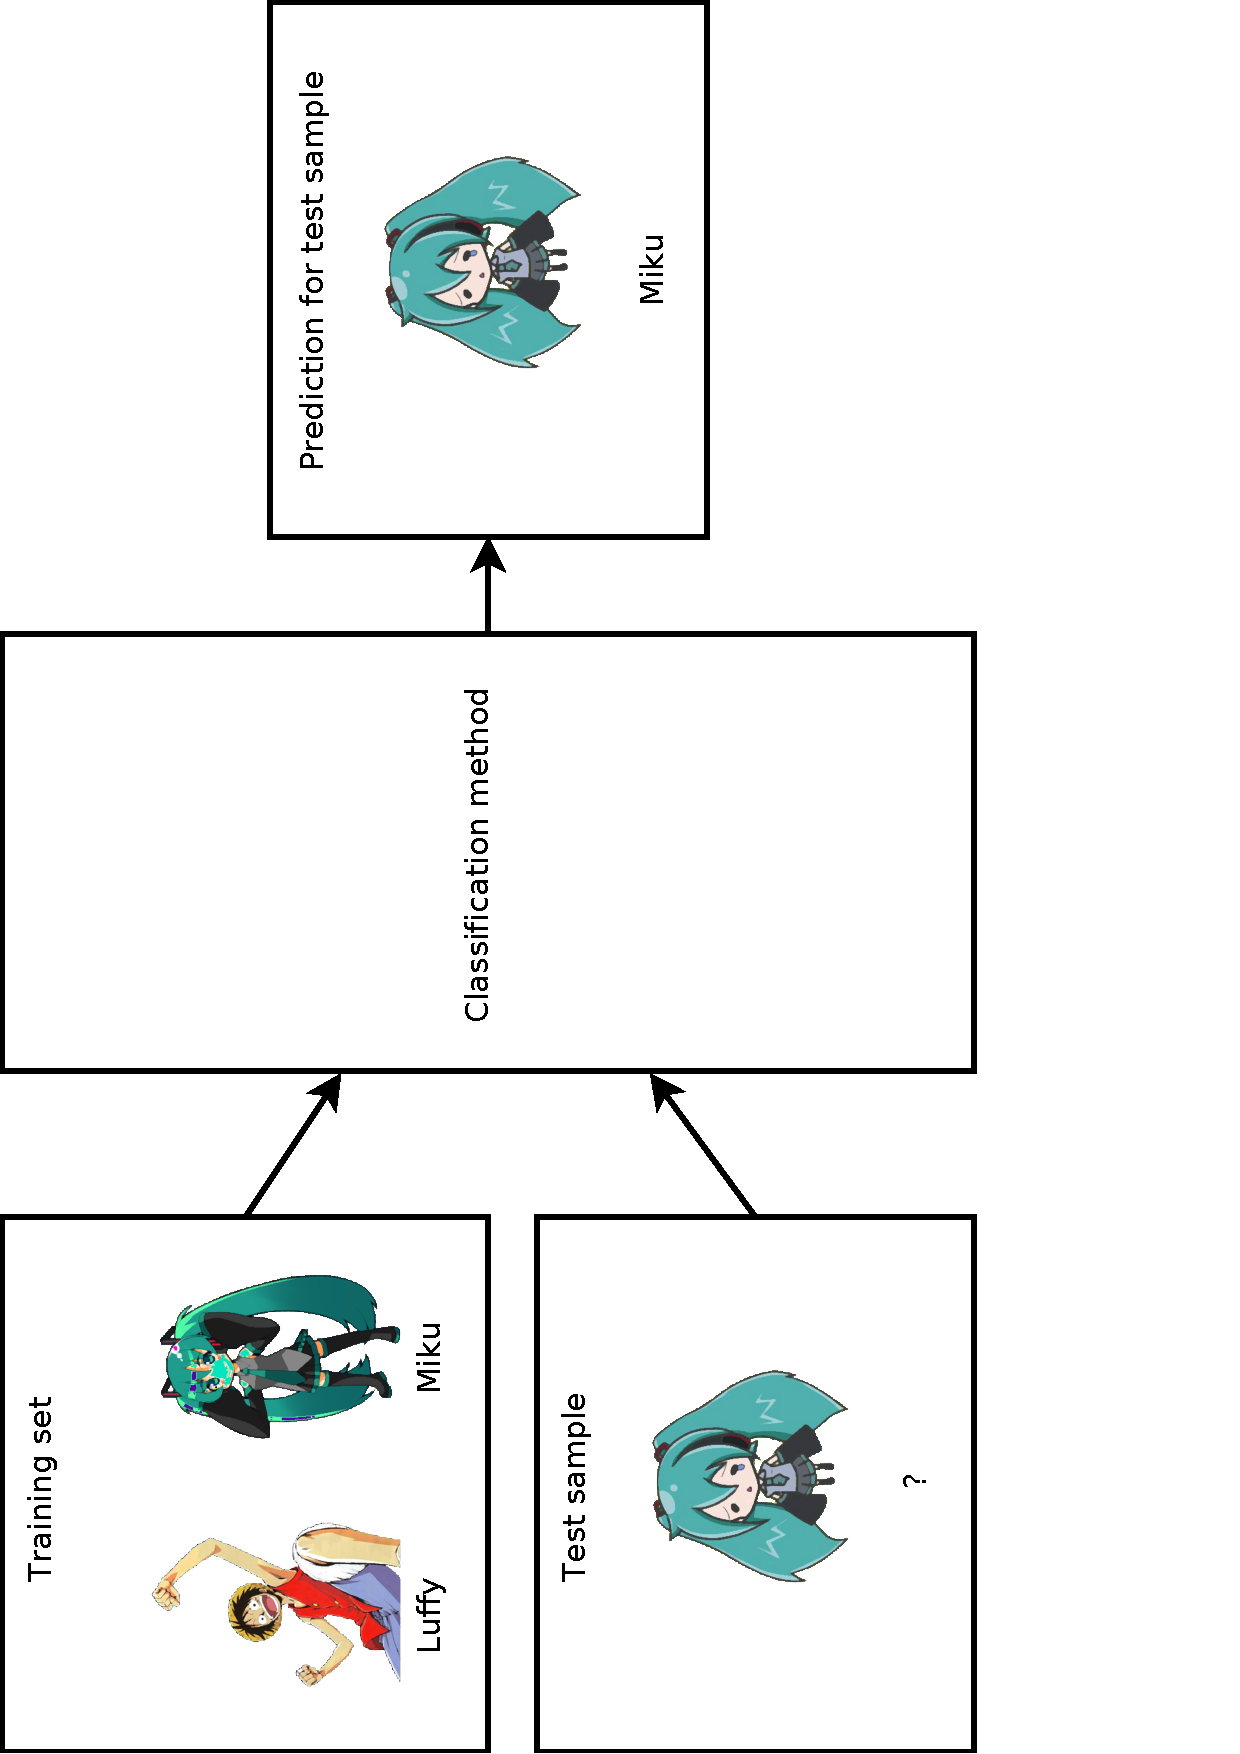
\includegraphics[height=1.2\textwidth, angle=270,clip=true,trim=0 0 4cm 0]{images/trainingPredictionDiagram.pdf}
}
\caption{Diagram depicting how training and prediction work for the method.}
\label{fig:trainingPredictionDiagram}
\end{figure}

The subject of my work here was to design a computer algorithm able to automatically identify characters from color images. It should take the shape of a supervised or semi-supervised classification method, meaning it should be able to identify an image by comparing it against a training set. Said training set may consist of labeled images - images which are known to depict a certain character - as well as unlabeled images in the case of semi-supervised classification (\autoref{fig:trainingPredictionDiagram}).

\section{Position in the laboratory}
I worked in the Sakamoto laboratory as a research student.
\section{Previous studies}
Previous work in the laboratory by graduate student Yuki Nakagawa on the animation character identification problem identified a segmentation method\cite{felzenszwalb2004efficient} and a classification method\cite{harchaoui2007image} for the problem. A dataset of animation character images was also previously constituted.
\section{Objectives}
The first objective was to design a method which would improve on the state of the art in animation character identification, in terms of recognition rate, clustering quality or run time performance. The envisioned application domain being automatic image annotation for web artist communities such as Pixiv\footnotemark[1]
\footnotetext[1]{
\url{www.pixiv.net} is a popular Japanese web artist community.
}
 or deviantArt\footnotemark[2],
\footnotetext[2]{
\url{www.deviantart.com} is a popular English speaking web artist community.
}
it should also be able to handle large datasets.
\section{Planning}